\chapter{Введение}
В данной работе был использован фреймворк Mr.LDA\cite{mrlda}, который основывается на модели Латентного 
размещения Дирихле (LDA).

\section{Модель LDA}
Латентное размещение Дирихле (LDA) -- это порождающая модель, позволяющая объяснять результаты наблюдений с 
помощью неявных групп, что позволяет получить объяснение, почему некоторые части данных схожи. Например, 
если наблюдениями являются слова, собранные в документы, утверждается, что каждый документ представляет 
собой смесь небольшого количества тем и что появление каждого слова связано с одной из тем документа. LDA 
является одним из методов тематического моделирования и впервые был представлен в качестве графической 
модели для обнаружения тематик Дэвидом Блеем, Эндрю Ын и Майклом Джорданом в 2003 году. \cite{bib:01}

Очевидно, что у одного документа может быть несколько тем; подходы, которые кластеризуют документы по темам, 
никак этого не учитывают. LDA -- это иерархическая байесовская модель, состоящая из двух уровней:
\begin{itemize}
    \item на первом уровне -- смесь, компоненты которой соответствуют <<темам>>;
    \item на втором уровне -- мультиномиальная переменная с априорным распределением Дирихле, 
        которое задаёт <<распределение тем>> в документе.
\end{itemize}

\begin{figure}[ht!]
    \center
    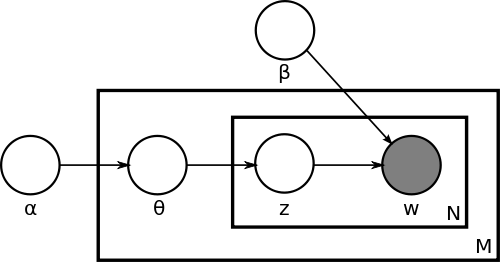
\includegraphics[width=0.47\textwidth]{lda}
    \caption{Граф модели}
\end{figure}

Сложные модели часто проще всего понимать рассмотрев на примере как модель будет генерировать новый документ:
\begin{itemize}
    \item выбрать длину документа \( N \) (этого на графе не нарисовано -- это не то чтобы часть модели);
    \item выбрать вектор \( \theta \sim (\alpha) \) -- вектор <<степени выраженности>> каждой темы в 
        этом документе;
    \item для каждого из \( N \) слов \( w \):
    \begin{itemize}
        \item выбрать тему \( z_n \) по распределению \( Mult(\theta) \);
        \item выбрать слово \( w_n \sim p(w_n | z_n, \beta) \) с вероятностями, заданными в \( \beta \).
    \end{itemize}
\end{itemize}

Для простоты мы фиксируем число тем \( k \) и будем считать, что \( \beta \) -- это просто набор параметров 
\( \beta_{i,j} = p(w^j = 1 | z^i = 1)\), которые нужно оценить. Совместное распределение тогда выглядит так:
\[
    p(\theta,\ldots,N|\alpha,\beta) = 
        p(N|\eta)p(\theta|\alpha)\prod\limits_{n=1}^{N}p(z_n|\theta)p(w_n|z_n,\beta)
\]
В отличие от обычной кластеризации с априорным распределением Дирихле или обычного наивного байеса, мы тут 
не выбираем кластер один раз, а затем накидываем слова из этого кластера, а для каждого слова сначала 
выбираем по распределению \( \theta \) тему, а уже потом набрасываем это слово по этой теме.

На выходе после обучения модели LDA получаются векторы \( \theta \), показывающие, как распределены темы в 
каждом документе, и распределения \( \beta \), показывающие, какие слова более вероятны в тех или иных 
темах. Таким образом, из результатов LDA легко получить для каждого документа список встречающихся в нём 
тем, а для каждой темы -- список характерных для неё слов, то есть фактически описание темы.\cite{lda}

\section{Фреймворк Mr.LDA}
Свободно распространяемый фреймворк Mr.LDA \cite{mrldainfo} является гибким и легко масштабируемым пакетом 
для многоязычного моделирования с использованием технологии MapReduce. Латентное размещение Дирихле (LDA) и 
связанная с ней техника моделирования по темам полезны для изучения коллекции документов. Из-за роста 
распространенности больших объемов данных, существует необходимость улучшить масштабируемость вывода для 
LDA. В отличие от других методов, которые используют выборку Гиббса, Mr.LDA использует вариационный метод, 
что легко подходит для использования в распределенной среде. Что еще более важно, эта вариационный метод, в 
отличие от трудно настраиваемой и специализированной реализации на основе выборки Гиббса, является 
легко расширяемым.

\newpage

\chapter{Установка}
В качестве базовой системы была выбрана Arch Linux \cite{arch}, основные возможности которого заключаются в 
\begin{itemize}
    \item гибкая настройка
    \item минимальный набор программ при установке
    \item большой репозиторий с программами \\
        \url{https://www.archlinux.org/packages/}, \url{https://aur.archlinux.org/}
    \item большое количество справочной документации\\
        \url{https://wiki.archlinux.org/}
\end{itemize}
Подробный гид по установке Arch Linux доступно по ссылке\\
\url{https://wiki.archlinux.org/index.php/Beginners%27_guide}.

\section{Виртуализация}
В качестве системы виртуализации был выбран VirtualBox за простоту в установке и настройке. Является 
многофункциональным инструментом для создания изолированных виртуальных машин, предлагает высокую 
производительность, а также является единственным профессиональным решением, которое находится в свободном 
доступе с открытым исходным кодом на условиях GNU General Public License (GPL) v.2.

VirtualBox активно развивается с частыми обновлениями и имеет постоянно растущий список функций, 
поддерживаемых гостевых операционных систем и платформ, с которыми он работает. Является результатом 
коллективной работы при поддержке выделенных компаний: каждому предлагается внести свой вклад, в то время 
как Oracle обеспечивает соответствие продукта профессиональным критериям качества. 

Так как VirtualBox не может предоставить максимальную возможную производительность для своих виртуальных 
машин. С увеличением количества расчётов растёт средний уровень издержек на их обработку, что крайне 
нежелательно для обработки больших данных и в том числе использование Hadoop. Поэтому в дальнейшем будет 
использовано одно из следующих решений, для уменьшения издержек:
\begin{itemize}
    \item система виртуализации Proxmox
    \item система виртуализации VMWare
    \item настройка и развёртывание Hadoop на основной системе
\end{itemize}

\section{Установка и настройка}
Предоставленные ноды работают на CentOS 6.5, в связи с этим установка виртульной машины была произведена из 
rpm пакета скаченного с официального сайта. Установка VirtualBox из репозитория не желательна, так как в 
этом случае будут установлены ненужные зависимости, такие как gui-оболочка.

\noindent\textbf{ВАЖНО} После установки необходимо добавить пользователя в группу \emph{vboxusers}:
\begin{lstlisting}
$ sudo usermod -aG vboxusers <name>
\end{lstlisting}
и запустить в терминале
\begin{lstlisting}
$ sudo /etc/init.d/vboxdrv setup
\end{lstlisting}
для установки и загрузки необходимых драйверов в ядро системы. Также желательным, но необязательным пунктом 
является установка так называемого Extension Pack для VirtualBox, рассмотрим установку на версии 4.3.24
\begin{lstlisting}
$ wget http://download.virtualbox.org/virtualbox/4.3.24/Oracle_VM_VirtualBox_Extension_Pack-4.3.24-98716.vbox-extpack
$ sudo BoxManage extpack install Oracle_VM_VirtualBox_Extension_Pack-4.3.24-98716.vbox-extpack
\end{lstlisting}

\section{Создание виртуальной машины в терминале}
Для создания виртуальной машины выполним следующую команду:
\begin{lstlisting}
$ VBoxManage createvm --name HadoopMaster --ostype ArchLinux_x64 --register
\end{lstlisting}
В случае успеха программа зарегистрирует виртуальную машину и выдаст ей UUID. Далее произведем настройку 
виртуальной машины
\begin{lstlisting}
$ VBoxManage modifyvm HadoopMaster --memory 16384 --audio none --nic1 nat \
    --natpf1 "ssh,tcp,,2468,,2468" --vram 4 --accelerate3d off \
    --boot1 disk --acpi on --cableconnected1 on --usb off
\end{lstlisting}
Используемые параметры:
\begin{itemize}
    \item memory -- количество оперативной памяти
    \item audio -- звук
    \item nic1 -- сеть, 
    \item natpf1 -- проброс портов
    \item vram -- количество видеопамяти
    \item accelerate3d -- поддержка ускорения 3d
    \item boot1 -- тип загрузки
    \item acpi -- управление питанием
\end{itemize}
Добавим контроллер HDD и подключим диск
\begin{lstlisting}
$ VBoxManage storagectl HadoopMaster --name "IDE Controller" --add ide
$ VBoxManage storageattach HadoopMaster --storagectl "IDE Controller" \
    --port 0 --device 0 --type hdd --medium <полный путь до файла vdi>
\end{lstlisting}
Теперь можно производить запуск виртуальной машины следующей командой:
\begin{lstlisting}
$ VBoxManage startvm HadoopMaster --type headless
\end{lstlisting}
Остановка производится следующей командой:
\begin{lstlisting}
$ VBoxManage controlvm HadoopMaster poweroff
\end{lstlisting}

\chapter{Настройка Hadoop}
Прежде чем развернуть Hadoop в режиме Cluster необходимо подготовить образ в режиме Single Node, а потом 
внести некоторые изменения.

\section{Режим Single Node}
\noindentСоздаём ssh ключ для безпарольного подключения
\begin{lstlisting}
$ ssh-keygen -t rsa -P ' ' -f ~/.ssh/id_rsa
\end{lstlisting}
Добавляем его в список авторизованных
\begin{lstlisting}
$ cat ~/.ssh/id_rsa.pub >> ~/.ssh/authorized_keys
\end{lstlisting}
Изменяем следующие строчки в hadoop-env.sh
\begin{lstlisting}
$ sudo vim /etc/hadoop/hadoop-env.sh
    export JAVA_HOME=/usr/lib/jvm/java-7-openjdk
    export HADOOP_LOG_DIR=/home/user/hadoop/log
    export HADOOP_SSH_OPTS="-p 2468"
\end{lstlisting}
Изменяем файлы \emph{core-site.xml}, \emph{yarn-site.xml}, \emph{mapred-site.xml}, \emph{hdfs-site.xml}
\begin{lstlisting}
$ sudo vim /etc/hadoop/core-site.xml
    <configuration>
        <property>
            <name>fs.defaultFS</name>
            <value>hdfs://localhost:9000</value>
        </property>
    </configuration>
$ sudo vim /etc/hadoop/yarn-site.xml
    <configuration>
    <property>
        <name>yarn.nodemanager.aux-services</name>
        <value>mapreduce_shuffle</value>
    </property>
    <property>
        <name>yarn.nodemanager.aux-services.mapreduce.shuffle.class</name>
        <value>org.apache.hadoop.mapred.ShuffleHandler</value>
    </property>
    </configuration>
$ sudo vim /etc/hadoop/mapred-site.xml
    <configuration>
        <property>
            <name>mapreduce.framework.name</name>
            <value>yarn</value>
        </property>
    </configuration>
$ sudo vim /etc/hadoop/hdfs-site.xml
    <configuration>
        <property>
            <name>dfs.replication</name>
            <value>1</value>
        </property>
        <property>
            <name>dfs.namenode.name.dir</name>
            <value>file:///home/user/hadoop/hdfs/namenode</value>
        </property>
        <property>
            <name>dfs.datanode.data.dir</name>
            <value>file:///home/user/hadoop/hdfs/datanode</value>
        </property>
    </configuration>
\end{lstlisting}
Теперь создадим необходимые папки и изменим режим доступа к ним
\begin{lstlisting}
$ mkdir -p /home/user/hadoop/hdfs/namenode
$ mkdir -p /home/user/hadoop/hdfs/datanode
$ sudo chown user:hadoop -R /home/user/hadoop
\end{lstlisting}
Подготовим и запустим Namenode
\begin{lstlisting}
$ /usr/lib/hadoop/bin/hdfs namenode -format
$ /usr/lib/hadoop/sbin/start-all.sh
\end{lstlisting}
В случае успеха при исполнении команды \emph{jps} получим следующее
\begin{lstlisting}
$ jps
6297 DataNode
1051 NameNode
1626 ResourceManager
7737 Jps
1143 SecondaryNameNode
\end{lstlisting}

\section{Режим Multi Node}
\noindentОтредактируем файл \emph{hosts}
\begin{lstlisting}
$ sudo vim /etc/hosts
    master 192.168.120.21
    slave1 192.168.120.22
    slave3 192.168.120.23
    slave4 192.168.120.24
\end{lstlisting}
Изменим имя для каждой ноде в файле hostname (на примере master-ноды)
\begin{lstlisting}
$ sudo vim /etc/hostname
    master
\end{lstlisting}
Произведём изменения в файлах \emph{core-site.xml}, \emph{yarn-site.xml}, \emph{mapred-site.xml} и \\
\emph{hdfs-site.xml}
\begin{lstlisting}
$ sudo vim /etc/hadoop/core-site.xml
    заменим localhost на master
$ sudo vim /etc/hadoop/hdfs-site.xml
    установим параметр dfs.replication в значение 3
$ sudo vim /etc/hadoop/yarn-site.xml
    добаим следующие строчк
    <configuration>
        <property>
            <name>yarn.resourcemanager.resource-tracker.address</name>
            <value>master:8025</value>
        </property>
        <property>
            <name>yarn.resourcemanager.scheduler.address</name>
            <value>master:8030</value>
        </property>
        <property>
            <name>yarn.resourcemanager.address</name>
            <value>master:8050</value>
        </property>
    </configuration>
$ sudo vim /etc/hadoop/mapred-site.xml
    заменим mapreduce.framework.name на mapred.job.tracker
    заменим yarn на master:54311
\end{lstlisting}
Сделаем копию главной ноды как (slave1, slave2, slave3, slave4). Измением имя для каждой ноды
\begin{lstlisting}
$ sudo vim /etc/hostname
    slave<номер ноды>
\end{lstlisting}
И удалим секцию содержащую \emph{dfs.namenode.name.dir} из файла \emph{/etc/hadoop/hdfs-site.xml}. Далее на 
главной ноде (master) добавим данные в следующие файлы
\begin{lstlisting}
$ sudo vim /etc/hadoop/masters
    master
$ sudo vim /etc/hadoop/slaves
    master
    slave1
    slave2
    slave3
    slave4
\end{lstlisting}
Произведём копирование ключей на все ноды
\begin{lstlisting}
$ sudo ssh-copy-id -i ~/.ssh/id_rsa.pub user@master
$ sudo ssh-copy-id -i ~/.ssh/id_rsa.pub user@slave1
$ sudo ssh-copy-id -i ~/.ssh/id_rsa.pub user@slave2
$ sudo ssh-copy-id -i ~/.ssh/id_rsa.pub user@slave3
$ sudo ssh-copy-id -i ~/.ssh/id_rsa.pub user@slave4
\end{lstlisting}
Подготовим и запустим Namenode
\begin{lstlisting}
$ /usr/lib/hadoop/bin/hdfs namenode -format
$ /usr/lib/hadoop/sbin/start-all.sh
\end{lstlisting}
В случае успеха при исполнении команды \emph{jps} получим на master-ноде следующее
\begin{lstlisting}
$ jps
6297 DataNode
1051 NameNode
1626 ResourceManager
7737 Jps
1143 SecondaryNameNode
\end{lstlisting}
А на slave-нодах
\begin{lstlisting}
$ jps
2362 DataNode
1089 NodeManager
5537 Jps
\end{lstlisting}

\chapter{Развёртывание Mr.LDA}
\section{Выполнение работы}
\noindentНа рабочую систему были установлены следующие программные компоненты:
\begin{itemize}
    \item Java Development Kit (jdk7-openjdk 7.u71\_2.5.3-1);
    \item Maven 3.3.3-1
    \item Scala 2.11.4-1;
    \item Apache Hadoop 2.7.2-1;
    \item Python 3.4.2;
\end{itemize}
А также дополнительные компоненты, идущие в зависимостях у этих пакетов.

Для работы с фреймворком была произведена компиляция исходного кода и был получена рабочая версия программы. 
Имя выходного файла: \emph{mrlda-0.9.0-SNAPSHOT-fatjar.jar}. Подробности по настройке и компиляции доступны 
по ссылке \url{https://github.com/lintool/Mr.LDA}.

Для преобразования данных патентов в рабочий формат фреймворка Mr.LDA, а также для экспорта данных в БД были 
использованы следующие программы написанные на языке Python:
\begin{itemize}
    \item программа для преобразования данных патентов в рабочий формат Mr.LDA и записи информации из 
        патентов в БД;
    \item программа для преобразования полученных данные от Mr.LDA и записи их в БД.
\end{itemize}
Исходные коды доступны по следующей ссылке:\\
\url{https://github.com/SemPatent/Golubev}

\section{Работа с Mr.LDA}
Подробное описание работы фреймворка Mr.LDA представлено в \cite{mrlda}. Рассмотрим главное по работе 
написанных программ и Mr.LDA.

Для работы программ необходимо следующее компоненты:
\begin{itemize}
    \item Python 3.4.2
    \item PostgreSQL
    \item Библиотека py-postgresql
    \item Библиотека xml
\end{itemize}

Для подготовки патентов для обработке на фреймворке Mr.LDA их необходимо преобразовать в его рабочий формат. 
Для этого был использована программа 
\href{https://github.com/SemPatent/Golubev/blob/master/convert_raw_patent.py}{convert\_raw\_patent.py}. На 
вход программы подаётся директория с файлами патентов в формате xml, а также имя выходного файла для Mr.LDA.
По завершению работы программы выходной файл можно передать на обработку Mr.LDA. 
\begin{lstlisting}
$ hadoop jar ./mrlda-0.9.0-SNAPSHOT-fatjar.jar cc.mrlda.ParseCorpus \
    -input <ИМЯ-ФАЙЛА> -output mrlda-parsed-data
\end{lstlisting}
По завершению индексации входного файла в текущей директории появится каталог \emph{mrlda-parsed-data} со следующей структурой.
\begin{lstlisting}
mrlda-parsed-data/document
mrlda-parsed-data/term
mrlda-parsed-data/title
\end{lstlisting}
Для запуска вариационного метода LDA используем следующую команду. 
\begin{lstlisting}
$ nohup hadoop jar ./mrlda-0.9.0-SNAPSHOT-fatjar.jar cc.mrlda.VariationalInference \
    -input mrlda-parsed-data/document -output mrlda-output-data \
    -term 10000 -topic 20 -iteration 50 -mapper 50 -reducer 20 >& lda.log &
\end{lstlisting}
Где основные флаги:
\begin{itemize}
    \item -term -- количество уникальных токенов в патенте
    \item -topic -- выборка документов
\end{itemize}
По завершению работы этой стадии выходные данные от Mr.LDA нужно преобразовать и записать в БД. Для этого 
нужно преобразовать внутренний формат Mr.LDA в текстовой следующими командами:
\begin{lstlisting}
$ hadoop jar ./mrlda-0.9.0-SNAPSHOT-fatjar.jar edu.umd.cloud9.io.ReadSequenceFile \
    mrlda-output-data/beta-ITERATION > mrlda.beta.file
$ $hadoop jar ./mrlda-0.9.0-SNAPSHOT-fatjar.jar edu.umd.cloud9.io.ReadSequenceFile \
    mrlda-output-data/alpha-ITERATION > mrlda.alpha.file
\end{lstlisting}
Где \emph{ITERATION} -- номер где LDA сходится. Для дальнейшего преобразования и экспорта в БД используется 
программа 
\href{https://github.com/SemPatent/Golubev/blob/master/convert_from_mrlda.py}{convert\_from\_mrlda.py}. На 
вход программы подаётся два файла \emph{mrlda.alpha.file} и \emph{mrlda.beta.file} полученные с помощью 
предыдущей команды.

\newpage

\chapter{Выводы}
В ходе работы была проделаны следующие работы:
\begin{itemize}
    \item подготовлены образы для виртуальной машины
    \begin{itemize}
        \item master
        \item slave
    \end{itemize}
    \item развёрнут набор программ для обработки патентов
    \begin{itemize}
        \item Hadoop
        \item PostgreSQL
        \item Python v3
    \end{itemize}
    \item настроен Hadoop в режиме Cluster node (неполная работоспособность)
    \item произведена первая итерация для обработки патентов -- подготовлен входной файл 
        для Mr.LDA и заполнена БД
\end{itemize}
В связи с проблема в настройке системы Hadoop был запущен на обработку только одном из несколько кластеров.
Данная проблема в проработке и будет решена в дальнейшей работе. Также на настройку и запуск системы 
повлияла непостоянная работы вычислительных нод.

В целом была произведена большая часть работы по подготовке и настройке оборудования и ПО. Результаты 
работы доступны по ссылке:\\
\url{https://mega.co.nz/#F!gplQFaYC!VE31z6vEx7pddy7lDPt70w}
Где доступны следующие файлы:
\begin{itemize}
    \item master\_image.tar.gz -- образ виртуальной машины master-ноды
    \item slave\_image.tar.gz -- образ виртуальной машины slave-ноды
    \item mrlda-input-file -- входной файлы для фреймворка Mr.LDA
    \item postgresql-backup.tar.bz2 -- backup базы данный
\end{itemize}

\newpage

\renewcommand{\bibname}{Информационные источники}
\addcontentsline{toc}{chapter}{Информационные источники}
\begin{thebibliography}{10}
    \bibitem{arch} Свободно распространяемый дистрибутив Arch Linux\\
        \url{https://archlinux.org/}
    \bibitem{archwiki} Вики документация по дистрибутиву Arch Linux\\
        \url{https://wiki.archlinux.org/}
    \bibitem{hadoop} Справочная документация по Apache Hadoop\\
        \url{http://hadoop.apache.org/docs/stable/}
    \bibitem{systemd} Демон инициализации systemd\\
        \url{http://www.freedesktop.org/wiki/Software/systemd/}
    \bibitem{mrlda} Репозиторий кода фреймворка Mr.LDA\\
        \url{https://github.com/lintool/Mr.LDA}
    \bibitem{lda} Habrahabr -- Рекомендательные системы: LDA\\
        \url{http://habrahabr.ru/company/surfingbird/blog/150607/}
    \bibitem{virtualbox} Программынй продукт виртуализации VirtualBox\\
        \url{https://www.virtualbox.org/}
\end{thebibliography}

\noindentИнформация по настройке Hadoop:\vspace*{-0.5em}
\begin{itemize}\itemsep-5pt
    \item Getting started with Hadoop in easy steps\\\footnotesize
        \url{http://www.thecloudavenue.com/2011/12/getting-started-with-hadoop-is-easy.html}
        \normalsize
    \item How to setup a Hadoop 2-node cluster on VirtualBox in less than an hour\\\footnotesize
        \url{https://gordoncluster.wordpress.com/2013/07/10/how-to-setup-a-hadoop-2-
        node-cluster-on-virtualbox-in-less-than-an-hour/}
        \normalsize
    \item Hadoop 2.6.0 Multi Node Cluster Setup on Ubuntu 14.10\\\footnotesize
        \url{http://chaalpritam.blogspot.ru/2015/01/hadoop-260-multi-node-cluster-setup-on.html}
        \normalsize
    \item Apache Hadoop 2.7.0\\\footnotesize
        \url{https://hadoop.apache.org/docs/r2.7.0/}
        \normalsize
\end{itemize}

\newpage

\renewcommand{\bibname}{Список используемой литературы}
\addcontentsline{toc}{chapter}{Список используемой литературы}
\begin{thebibliography}{10}
    \bibitem{bib:01} Blei,~D.~M Latent Dirichlet Allocation ~/ David M. Blei, Andrew Y. Ng, 
        Michael I. Jordan~// Available at: http://www.jmlr.org/papers/volume3/blei03a/blei03a.pdf
    \bibitem{mrldainfo} Zhai,~K. Mr. LDA: A Flexible Large Scale Topic Modeling Package using Variational 
        Inference in MapReduce~/ Ke Zhai, Jordan Boyd-Graber, Nima Asadi~//
        Available at: http://www2012.org/proceedings/proceedings/p879.pdf
\end{thebibliography}